%% Alkuperäinen lähde: LaTeX-mallidokumentteja - Turun yliopisto, Matematiikan ja tilastotieteen laitos
%% https://www.utu.fi/fi/yksikot/sci/yksikot/mattil/opiskelu/latex/malleja/Sivut/home.aspx
%% Modifioitu:
%% 10/20017 Turun yliopisto, Tulevaisuuden teknologioiden laitos; Elise Syrjälä
%% parannusehdotuksia otetaan mielellään vastaan

\documentclass[12pt, titlepage]{article}
\usepackage[a4paper,bindingoffset=0.2in,%
            left=1in,right=1in,top=1in,bottom=1in,%
            footskip=.25in]{geometry} %% Lisätty uuteen versioon marginaalien asettelu
\usepackage{amssymb,amsthm,amsmath} % ams
\usepackage[finnish]{babel} % suomenkielinen tavutus
\usepackage[T1]{fontenc} % skanditavutus
\usepackage[utf8]{inputenc} % skandit utf-8 koodauksella
%\usepackage[ansinew]{inputenc} % skandit utf-8 koodauksella, kokeile tata, jos utf-8 ylla ei toimi.

\usepackage{graphicx} % dokumentti sisaltaa kuvia

\linespread{1.24} %rivivali 1.5
\sloppy % Vahentaa tavutuksen tarvetta, "leventämalla" rivin keskella olevia välilyöntejä.

%% Lauseille, maaritelmille ja muille vastaaville voidaan maaritella omat ymparistöt
%% jolloin niille saadaan yhtenainen ulkoasu
\theoremstyle{definition}
\newtheorem{maar}{Maaritelma}[section] %Numeroidaan maaritelmat yms lukukohtaisesti. Juoksevan numeroinnin saa jattamalla [section]-option pois
\newtheorem{lemma}[maar]{Lemma} % Tässä ymparistö 'lemma' käyttää laskuria 'maaritelma'
%\newtheorem{lemma}{Lemma}[section] %Ymparistölle 'lemma' voitaisiin määritella myös oma laskurinsa.
\newtheorem{lause}[maar]{Lause}
\newtheorem{esimerkki}[maar]{Esimerkki}

%% Yleisimmin kayttettaville komennoille voi maaritella lyhynnemerkintöja
%% esimerkiksi
\newcommand{\Q}{\mathbb{Q}}
\newcommand{\R}{\mathbb{R}}
\newcommand{\Z}{\mathbb{Z}}
\newcommand{\C}{\mathbb{C}}
\newcommand{\abs}[1]{\vert #1 \vert} % Itseisarvo

%% === Täytä tiedot ===

%% Muuta seuraavat tiedot omaan tutkielmaasi sopiviksi
%% Päivitä ja aktivoi sopiva
\title{Lisää otsikko tänne \\ {\normalsize
LuK-tutkielma, Tietojenkäsittelytiede}}


%\author{Etunimi Sukunimi \\[0.3cm] LuK-/TkK-tutkielma\\[0.3cm] Tietojenkäsittelytiede } %suuremmalla välillä
%% Täytä
\author{Vieno Väistönen}
\date{Joulukuu 2017}
%%%%%%%%%%%%%%%%%%%%%%%%%%%%%%

\makeatletter
\let\inserttitle\@title
\let\insertworktype\@worktype
\makeatother

\makeatletter
\let\insertauthor\@author
\makeatother

\makeatletter
\let\insertdate\@date
\makeatother

\begin{document} % Dokumentti alkaa

\pagestyle{empty} % Ei sivunumerointia etusivulla ja sisällysluettelossa

\vspace*{\fill} % Otsikkotietojen asettaminen sivun keskelle
\begin{center}\Large %
\inserttitle
\end{center}

\vspace{0.3cm}
\begin{center}
\insertauthor \\
\insertdate
\end{center}

\vfill % Sivun alaosan tiedot ihan alaosaan
\begin{center}
TURUN YLIOPISTO\\
Tulevaisuuden teknologioiden laitos\\
\end{center}

%% === Turnit ===
\begin{center}
\noindent {\footnotesize Turun yliopiston laatujärjestelmän mukaisesti tämän julkaisun alkuperäisyys on tarkastettu Turnitin OriginalityCheck -järjestelmällä.}
\end{center}

\newpage % Uusi sivu
\tableofcontents %Tehdaan tahan sisällysluettelo

\newpage

%% Aloitetaan sivunumerointi
\pagestyle{plain}
\setcounter{page}{1}

\section{Johdanto}

Työ ei perustu kirjaan \cite{latexcompanion}.

\section{Ymparistöjen kayttö}

\subsection{Maaritelmia}
\begin{maar}[Jatkuva funktio] Funktio $f:\R \rightarrow \R$ on jatkuva, jos jokaista positiivilukua $\varepsilon$ kohti on olemassa sellainen
positiiviluku $\delta$, etta mikali $\abs{x-x_0} <\delta $, niin $\abs{f(x)-f(x_0)}<\varepsilon.$
\end{maar}

\subsection{Apulauseita ja lemmoja}
Esitetaan todistuksetta \emph{Differentiaalilaskennan valiarvolause}.
\begin{lemma}[Differentiaalilaskennan valiarvolause]
\label{diffval}
Jos funktio $f$ on jatkuva suljetulla valilla $[a,b]$ ja derivoituva avoimella valilla $(a,b)$, niin on olemassa sellainen piste $\xi$ avoimella
valilla $(a,b)$, etta
\begin{equation}
\label{kaava1}
f'(\xi)=\frac{f(b)-f(a)}{b-a}.
\end{equation}
\end{lemma}

\subsection{Lauseita ja todistuksia}
Lemman \ref{diffval} avulla voidaan todistaa \emph{integraalilaskennan valiarvolause}.
\begin{lause}[Integraalilaskennan väliarvolause]
\label{intval}
Jos funktio $f$ on jatkuva suljetulla välillä $[a,b]$, niin on olemassa sellainen piste $\xi$ avoimella välillä $(a,b)$, että
\begin{equation}\label{kaava2}
\frac{1}{b-a}\int_a^b f(x)dx=f(\xi).
\end{equation}
\end{lause}
\begin{proof}
Asetetaan
\begin{equation*}
F(x)=\int_a^x f(t)dt
\end{equation*}
ja sovelletaan lemmaa \ref{diffval} tahan funktioon; $F(x)$ toteuttaa selvästi lemman oletukset. Koska $F'(x)=f(x)$, niin kaavan \eqref{kaava1} vasen
puoli on $f(\xi)$. Koska $F(b)=\int_a^b f(t)dt$ ja $F(a)=0$, niin kaavan \eqref{kaava2} oikean puolen osoittaja on $F(b)-F(a)=\int_a^b f(t)dt$. Nain
ollen kaava \eqref{kaava1} tulee muotoon
\[%lyhennysmerkintä \begin{equation*}
f(\xi)=\frac{\int_a^b f(t)dt}{b-a}.
\] %lyhennysmerkintä \end{equation*}
\end{proof}

\section{Asia}

\subsection{Taulukot ja kuvat}

Joskus voi olla tarpeen tehdä taulukko. Taulukoissa \ref{taulukko1} ja \ref{taulukko2} on kummia arvoja. Table-ympäristössa \LaTeX sijoittaa taulukon parhaaksi katsomallaan tavalla. Taulukkoon saa tällöin myös kuvatekstin ja viittausnimen.
\begin{table}[!h] %Optio h määrittelee taulukon sijaintia (Here, Top, Bottom, Page)
\begin{center}
\begin{tabular}{|lr||c}%solujen tasaukset left right center
$k$& $n$ & $m$\\
\hline
1 & 2 & 3\\
4 & 5 & 6\\
$f(x)$ & teksti & 7\\
\end{tabular}
\caption{Kummia lukuja pystyviivoilla höystettynä}\label{taulukko1}
\end{center}
\end{table}

Vertailun vuoksi toinen taulukko, jossa käytetty samaa aineistoa eri muotoilun kanssa.

\begin{table}[!h] %Optio h määrittelee taulukon sijaintia (Here, Top, Bottom, Page)
\begin{center}
\begin{tabular}{llc}%solujen tasaukset left right center
$\textbf{k}$& $\textbf{n}$ & $\textbf{m}$\\
\hline
1 & 2 & 3\\
4 & 5 & 6\\
$f(x)$ & teksti & 7\\
\end{tabular}
\caption{Kummia lukuja yhdellä vaakaviivalla ja tummennetulla otsikorivillä}\label{taulukko2}
\end{center}
\end{table}

%% Tabular-käskyä vastaa matematiikkatilassa array.

Kuville taas voi käyttää figure-ympäristöa kuten on tehty kuvassa \ref{kuva}.
\begin{figure}[h!]
\begin{center}
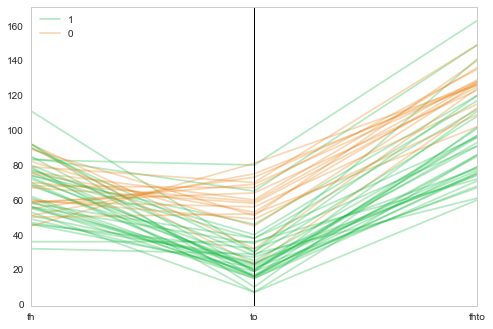
\includegraphics[width=0.6\textwidth]{figure_esimerkki.png}
\caption{Esimerkki kuvan upottamisesta dokumenttiin}
\label{kuva}
\end{center}
\end{figure}

\subsection{Matriiseja ja muita}
Käskyparilla left ja right ja tehtya sulkuja, joiden koko on sovitettu käskyparin väliin jäävan kokonaisuuden mukaan:
\[
\left(
\begin{array}{ccc}
a & b & c \\
d & e & f \\
g & h & i
\end{array}
\right)
\]

\[
\abs{x} =
\left\{
\begin{array}{rl}
x & \text{kun } x >0 \\
-x & \text{kun } x <0
\end{array}
\right.
\]

%% Viitteet

%Oletuksena Latex antaa kirjallisuusluettelolle nimen "Viitteet". Alla olevilla käskyillä tämän voi vaihtaa:

\addcontentsline{toc}{section}{Kirjallisuutta} %sisällysluetteloon
\renewcommand{\refname}{Kirjallisuutta} %otsikon muutos

%% -- Viitteet tapa 1 --
%% Viitteet dokumenttitekstissä

%% Viitteet täältä: https://www.sharelatex.com/learn/Bibliography_management_with_bibtex
\begin{thebibliography}{9}
\bibitem{latexcompanion}
Michel Goossens, Frank Mittelbach, and Alexander Samarin.
\textit{The \LaTeX\ Companion}.
Addison-Wesley, Reading, Massachusetts, 1993.

\bibitem{einstein}
Albert Einstein.
\textit{Zur Elektrodynamik bewegter K{\"o}rper}. (German)
[\textit{On the electrodynamics of moving bodies}].
Annalen der Physik, 322(10):891–921, 1905.

\bibitem{knuthwebsite}
Knuth: Computers and Typesetting,
\\\texttt{http://www-cs-faculty.stanford.edu/\~{}uno/abcde.html}, (luettu 9.10.2017).
\end{thebibliography}
%% ------

%% -- viitteet tapa 2 --
%% Viitteet .bib-tiedostona

%% tuo .bib-tiedosto manuaalisesti files->Bibliography

%% Valitse haluamasi tyyli tai lisää sopiva, aputekstin tyyliselvitys Overleaf+Mendeley -yhdistelmälle
% \bibliographystyle{plain} %viittaukset numeroina, viitteet määrittelyjärjestyksessä
% \bibliographystyle{apalike} %viittaukset nimi+vuosi, viitteet aakkosjärjestyksessä
%\bibliographystyle{unsrt} %viittaukset numeroina, viitteet esiintymisjärjestyksessä

%% .bib-tiedoston nimiosa, eli tämä viittaa tiedostoon kandiviitteet.bib
% \bibliography{kandiviitteet}


%% Vinkki: jos käytät esimerkiksi Mendeley-palvelua, niin files->Bibliography antaa mahdollisuuden automaattiseen .bib-tiedoston päivittämiseen
%% ------

%% dokumentti loppuu
\end{document}
